%!TEX root = ../thesis.tex
%*******************************************************************************
%****************************** Second Chapter *********************************
%*******************************************************************************

\chapter{Deep learning}

\ifpdf
     \graphicspath{{Figs/Chapter2/}}
\else
    \graphicspath{{Chapter2/Figs/Vector/}{Chapter2/Figs/}}
\fi

There are many tasks which are hard to write algorithms for. For example, writing an algorithm that identifies a type of fruit in a picture of the fruit is a challenging undertaking. One could try to do this by asking a number of yes or no questions to help whittle down the possibilities. Sensible questions might be: "is the fruit round?", "is the fruit green?", and "is the fruit's surface rough?". The problem with this approach is that it is very brittle. More questions could be introduced to disambiguate more cases, but the large variations in the appearance of fruit can cause the algorithm to become confused. Writing rules in this way is also not scalable. There are many types of fruits, and writing questions to determine each one quickly becomes intractable. \par
 
\noindent Machine learning (ML) can be used to solve such tasks, as well as others like weather prediction, stock price forecasting and risk modelling \unskip ~\citep{hastie2009elements}. ML is the process of using data to build prediction models, where these models typically output discrete (classification) or continuous (regression) values. There are various learning paradigms \unskip ~\citep{murphy2012machine}, including supervised learning, unsupervised learning and reinforcement learning, to train models from data in order to perform a specific task. The models can be divided into three classes, namely shallow, deep and probabilistic ~\citep{hastie2009elements, murphy2012machine}. \par

\noindent This chapter presents a discussion on the supervised learning paradigm, a description of deep convolutional \unskip ~\citep{lecun1998gradient} and recurrent network \unskip ~\citep{werbos1988generalization} neural network models, and a discussion on regularisation techniques for deep models, including dropout \unskip ~\citep{srivastava2014dropout} and batch normalisation \unskip ~\citep{ioffe2015batch}. 


%********************************** %First Section  **************************************

\section{Supervised learning}

An ML prediction model takes as input a set of features. These features are attributes of a data sample. For example in the fruit prediction task mentioned above, input features might be characteristics such as shape, colour, texture and size. These inputs are provided to a model that maps them to outputs. In the example above, these outputs would be types of fruit, and could represent values such corresponding to orange, apple, strawberry, pineapple, etc. The model is then trained to identify the correct fruit (output) based on the features (input) it receives, from a collection of input-output examples, a type of training called supervised learning \citep{bishop2006pattern, hastie2009elements, murphy2012machine}.

\begin{figure}[H]
   	\centering
    	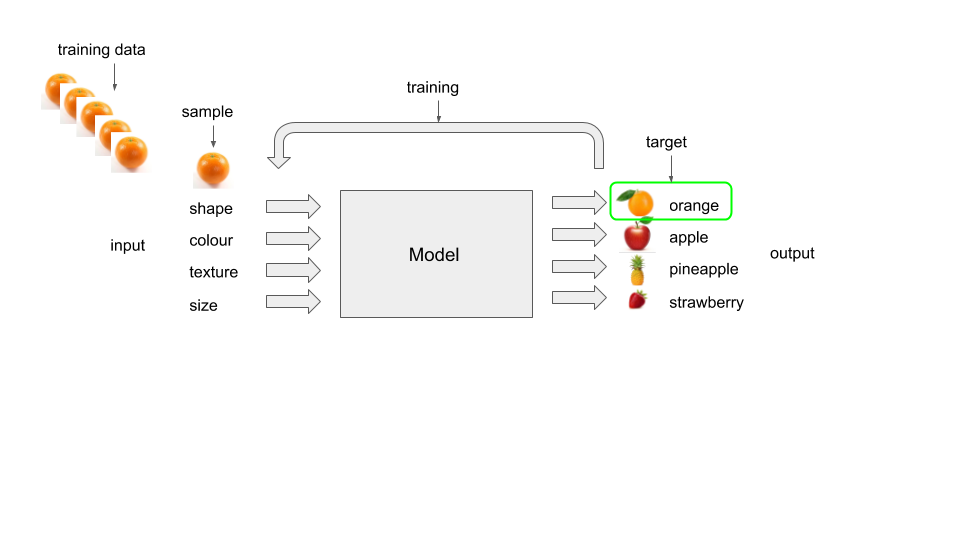
\includegraphics[width=\textwidth]{supervised_learning}
	\caption{A supervised learning model is trained to map input features to expected output.}
\end{figure}

\noindent Features can be continuous valued or discrete, where discrete values are referred to as categorical variables. Outputs can also be continuous or discrete, where discrete outputs are known as classes. Example input-output pairs comprise a training dataset which is represented as, \begin{math} D = \{(x_i, y_i)\}_{i=1}^N \end{math}, where \begin{math} D \end{math} is an dataset, \begin{math} x_i \end{math} is the input feature and \begin{math} y_i \end{math} is its expected output label. The model has to learn a general mapping from input features to output labels. \par

\noindent In the fruit example, the model will attempt to build decision boundaries between fruit classes in the feature space. We can visualise this process in a 2-dimensional setting using two fruit features, say shape and colour. Figure 2.2 shows an example of synthetically generated samples in this 2D feature space and a potential decision boundary.

\begin{figure}[H]
   	\centering
    	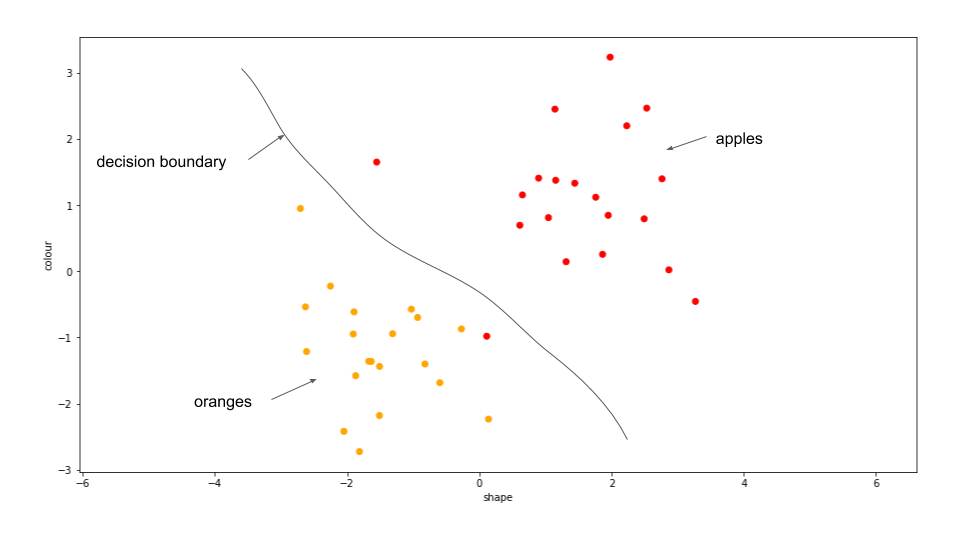
\includegraphics[width=0.8\textwidth]{oranges_and_apples_decision_boundary}
	\caption{A model decision boundary between two classes.}
\end{figure}

\noindent Data is assumed to be generated by the same underlying process, and is divided into two classes: independent and identically distributed (IID), and non-IID. In the context of IID data, samples are independent and therefore order invariant; whilst in the context of non-IID data, samples are dependent and order matters. The class of data can determine the best choice of model for prediction. \par

\noindent Training data is typically subdivided into three sets: training, validation and test. The training set provides in-sample data - input-output pairs which are exposed to the model during training and used to update its parameters. The validation set approximates out-of-sample data used to adjust model architecture, as well as hyperparameters (meta model parameters which configure its operation). The test set is used to assess the models prediction performance after training is complete. These results establish an objective measure of the model's utility.  \par

\noindent An objective function is used to measure the prediction performance of a model during training, and can compute an error or reward signal. When the objective computes an error, it is called a loss function, which measures the difference between the model's predicted output and the target output (the labels in the training set). As the model parameters are updated during training, the loss value changes and produces a multidimensional loss surface. The training algorithm tries to minimise this loss using a method of optimisation, such as bayesian, evolutionary or first order \unskip ~\citep{hastie2009elements, bishop2006pattern, murphy2012machine}. \par

\noindent A popular method of optimisation is gradient decent, an approach which attempts to descend to the lowest region of the loss surface: the global minimum. Model parameter updates are computed based on partial derivatives of the loss with respect to the individual parameter. The magnitude of the update is dependent on the magnitude of the loss i.e. the bigger the error, the bigger the update. A training algorithm uses such an optimsation method to guide the loss toward the global minimum, but in practice a local minimum is usually the best that can be achieved. This process in turn tries to guide the model toward a representative approximation of the underlying distribution of the data, enabling it to make predictions. \par

\noindent During training, mini-batch optimisation is used along with gradient descent to update model parameters. In mini-batch optimisation, the training set is divided into batches, where model parameters are updated after a mini-batch has been processed. This is in contrast to stochastic gradient descent where parameters are updated per sample, and batch gradient descent where parameters are updated after a run through the entire training set. Mini-batch optimisation is both robust to convergence (not as susceptible to local optima), and compute efficient. \newline
The supervised learning training algorithm is expressed as follows: \par 

\bigskip

\begin{algorithm}[H]
	\SetAlgoLined
	\textbf{Input} 
	Training set \begin{math} D = \{(x_i, y_i)\}_{i=1}^N \end{math}, of input features and output labels\;
	Intialise parameters $w \in \mathbb{R}$, for model \begin{math} M(w) \end{math} // e.g. random normal initialisation \\
	\For{Epoch \begin{math} k,  k \in [1, K]  \end{math}}{
  		\begin{math} S_{batch} \gets sample(D, b) \end{math} // sample minibatch of size \begin{math} b \end{math} \\
	 	\For{(x, y) \begin{math} \in S_{batch} \end{math}}{
     			\begin{math} y' \gets predict(x, \; y') \end{math} // predict label for sample \\
			\begin{math} e \gets y' - y \end{math} // compute loss
     			}
		$ w \gets w - \lambda * \hat{\nabla}_{w} J_{e} (w)$ // partial derivative update of model with respect to cost $e$
	}
	\caption{Supervised Learning}
\end{algorithm} \bigbreak


%********************************** %Second Section  **************************************

\section{Deep learning models}

Deep learning models have become popular for classification and regression tasks, and machine learning tasks in general. The reason for this is that deep models solve a major problem with shallow models, which is to select the best features with which to represent raw input samples \unskip ~\citep{Goodfellow-et-al-2016}. The problem of feature selection had resulted in a methodology used during shallow model development, called feature engineering. It includes techniques such as bucketing, crossing, hashing and embedding \unskip ~\citep{murphy2012machine, Goodfellow-et-al-2016}. These techniques are designed to build feature representations that will result in high classification and regression accuracy. Deep models attempt to discover optimal representations automatically during training, hence their superior performance on a number of machine learning tasks. \par

\noindent Multilayer perceptrons (MLPs) are deep learning models implemented as feed-forward neural networks, consisting of $N$ layers applied to an input vector $ x $. These models compute un-normalised scores, known as logits, for each of the possible outputs. MLPs construct a composition of nonlinear functions which describe an analytical definition of the generative process of the data used to train them. The utility of composition is what gives them the capability needed to model complex datasets. MLPs achieve nonlinear expressiveness with the use of nonlinear activation functions, including the ReLU, Sigmoid and Tanh function \unskip ~\citep{Goodfellow-et-al-2016}.  \par

\noindent MLPs produce output by executing a number of steps in what is called a forward pass, where each step is represented as a layer. A basic MLP may consist of three of these layers, an input, hidden and output layer. An MLP computes a linear combinations of input features, then transforms the representation using a nonlinear hidden activation layer, then pass the result to the next layer where linear combinations and nonlinear activations are performed. The forward pass can be expressed as follows:
\begin{subequations}
	\begin{gather}
		f_0 = x \\
		f_i=\sigma_i(W_if_{i - 1} + b_i) \quad i \in [1, N]
	\end{gather}
\end{subequations}

\noindent Each layer has a particular number,  $m_i$, of neurons. The parameters of a layer consist of a matrix $W_i \in \mathbb{R}^{m_i \times m_{i-1}}$ and bias vector $b_i \in  \mathbb{R}^{m_i}$. Each layer also has a nonlinear activation function $\sigma_i$. 

\noindent Loss functions are used to train deep models under a supervised learning paradigm. The error computed by the loss is used in a process called backpropagation. This process involves the computation of first order partial derivatives, and the adjustment of the parameters in a direction and magnitude relating to their respective derivative. In a network with $ L $ layers, the gradient for the respective parameter in layer $ i $ is given by:
\begin{subequations}
	\begin{gather}
		\frac{\partial E} {\partial W_i} = \frac{\partial E} {\partial z_L}\frac{\partial z_L} {\partial z_{L - 1}}  \dots \frac{\partial z_{i + 2}} {\partial z_{i + 1}}\frac{\partial z_{i + 1}} {\partial W_{i}} \\
		\frac{\partial E} {\partial b_i} = \frac{\partial E} {\partial z_L}\frac{\partial z_L} {\partial z_{L - 1}}  \dots \frac{\partial z_{i + 2}} {\partial z_{i + 1}}\frac{\partial z_{i + 1}} {\partial b_{i}}
	\end{gather}
\end{subequations}

\noindent where $ E $ is the cost function at the output (the aggregation of loss scores depending on stochastic, batch or mini-batch optimisation strategy), $ W_i $ is an intermediate weight matrix mapping inputs from layer $ i $ to outputs $ z_{i + 1} $  at layer $ i + 1 $, $ z $ is the un-normalised value produced by the layer output (known as the logit), $ b_i $ is the bias at layer $ i $. The matrix $ \frac{\partial z_{i + 1}} {\partial W_i} $ is called a Jacobian matrix. The Jacobian is a matrix contains the partial derivatives of the layer-specific parameters, with respect to the loss contributed by each parameter to the overall output error. It summarizes all the ways in which changing the matrix $ W_i $ by a small amount will influence the output $ z_{i + 1} $. The matrix is expressed as follows: \par
\begin{equation}
	\renewcommand\arraystretch{2}
	\mathbb{J} = \begin{bmatrix}
        		\frac{\partial z^1}{\partial W^1} & \frac{\partial z^2}{\partial W^1} & \cdots & \frac{\partial z^m}{\partial W^1} \\
           	\frac{\partial z^1}{\partial W^2} &\frac{\partial z^2}{\partial W^2} & \cdots & \frac{\partial z^m}{\partial W^2} \\
           	\vdots & \vdots & \ddots & \vdots \\
           	\frac{\partial z^1}{\partial W^n} & \frac{\partial z^2}{\partial W^n} & \cdots & \frac{\partial z^m}{\partial W^n} \\
        \end{bmatrix}
\end{equation}

\medskip
\noindent Different schemes are used to initialise layer parameters $ W_i $. These schemes are sensitive to the choice of activation function, $ \sigma_i $, used. Sigmoid and Tanh functions can saturate if parameters are intialised with values that are too large, or can die if intialised with values which are too small; which in turn can lead to exploding and vanishing parameter gradients. In order to overcome this problem Xavier intialisation \unskip ~\citep{glorot2010understanding} is used, which tries to scale the the parameters by the number of layer inputs and outputs. This limits the variance of layer outputs and helps stabilise gradient updates. When the ReLU activation is used He intialisation \unskip ~\citep{he2015delving}, a modification of Xavier initialisation, is commonly applied. \par

\noindent Together the forward pass algorithm and backpropagation, implicitly allow the automatic discovery of the most meaningful representation to compute the model output. We refer the reader to \unskip ~\citep{Goodfellow-et-al-2016} for a review on loss functions, as well as a more detailed discussion on the forward pass and backpropagation. 

%********************************** %Convolutional Networks  **************************************

\subsection{Convolutional networks}

MLPs suffer from an explosion of parameters  ~\citep{krizhevsky2012imagenet}. In an MLP layer, all features of an input vector are fully connected to all other features when computing the layer output. The outputs of a layer are then all fully connected to each other in the following layer. This interconnectedness causes the number of model parameters to grow exponentially in the number of input features. For example, a feed-forward network with two hidden layers consisting of $512$ and $256$ neurons respectively, an output size of $10$, and an input vector of shape $\left [ \begin{matrix} 200 \times 1 \end{matrix} \right] $, ends up with a total of $236,810$ parameters. This can cause a problem with high dimensional input vectors such as images, where input features may consist of a 3-dimensional input volume. MLPs may also need to be composed of a number of layers in order to produce satisfactory prediction performance when presented with high dimensional inputs. In such a scenario, parameters can number in the millions, resulting in a model that is computationally inefficient to train. \par

\noindent MLPs are also not able to take advantage of structure in data. When images are represented in a 2-dimensional matrix, common shapes may appear in a regular composition. For example, different cars may appear regularly as a compositions of rectangles and circles. The multiplication operator between the input matrix (or flattened input vector) and layer parameters of an MLP destroys the spatial information of the data, making the task of learning distributions of representations harder. In order to posses sufficient learning capacity that adequately models distributions of structural representations, MLPs need to be larger \unskip ~\citep{lecun1998gradient} and may still produce poor prediction performance. \par

\noindent Convolutional neural networks (CNNs) have been developed to overcome both the above mentioned problems experienced by MLPs. CNNs make use of the convolutional operator during representation learning, instead of the multiplication operator. This operator performs a convolutional operation on an input using a filter, a 2-dimensional matrix with trainable parameters. This process generates a latent feature map which is used in subsequent layers in the network. Latent feature maps capture structural patterns in data, building simple intermediate representations. CNNs compose these representations into more sophisticated representations in subsequent layers. \par 

\noindent The convolutional operator allows CNNs to capture translation invariance in inputs due to filter parameter sharing \unskip ~\citep{simonyan2014very}. Translation invariance allows the CNN to build an intermediate representation that is consistent under transformation, for example if an image is moved, that would lead to a consistent feature map representation being generated. This property allows CNNs to model the distribution of inputs using fewer parameters and smaller datasets. The trade off one makes when using CNNs is reduced flexibility in modelling complex decision boundaries. To mitigate this trade off, CNNs are often implemented with a final set of fully connected layers, in order to facilitate the expressiveness required for accurate prediction. In the following we discuss the CNN forward pass. \par

\noindent \textbf{Convolutional layers.} Convolutional layers rely on filters that are small spatially (along width and height), but extends through the full depth of an input volume. During the forward pass, each filter is convolved across the width and height of the input volume, where the element-wise dot product is computed between the entries of the filter and the input at a particular position. A 2-dimensional feature map is generated, that gives the responses of that filter at every spatial position of the input. Every convolutional layer has a set of filters, and each of them produces separate 2-dimensional feature maps, which are then stacked along the depth-dimension to produce an output volume. The size of the output volume is controlled by the hyperparameters of the convolutional layer: the filter size defines the width and height of the filters in the layer (filters always have the same depth as their input volume); the depth of the layer which defines the number of filters in the layer; the stride which defines the number of entries by which we move the filter when convolving it along the input volume; and padding which refers to the number of 0 entries we add to the input volume along the width and height dimensions. This padding parameter is useful in that it gives us more control over the desired size of the output volume and can be used to ensure that the output volume has the same width and height as the input volume \unskip ~\citep{DLIndaba2017}. Convolution of an input volume $X$ with a single filter $W$ is given by: 
\begin{equation}
	O_{ij}^{d} = b_d + \sum_{a=0}^{F - 1}\sum_{b=0}^{F - 1}\sum_{c=0}^{I - 1}W_{a,b,c,d}X_{i+a,j+b,c}^{pad}
\end{equation}

\noindent where $O_{ij}^d$ is the value of the output volume at position $(i,j,d)$, $b$ bias vector of shape $\left [ \begin{matrix} D \end{matrix} \right]$, $W$ is the weight tensor of shape $\left [ \begin{matrix} F \times F \times I \times D \end{matrix} \right]$, $X^{pad}$ is the padded input volume and $a, b, c$ are indices into the volume dimensions. \par

\noindent \textbf{Pooling layers.} A pooling layer is used to reduce the spatial size of the representation, in order to reduce the number of parameters in the network. Pooling layers provide latent features deeper in the network with a larger receptive field. In particular, pooling gives deeper latent features much larger receptive fields so that they can effectively combine smaller features together. Pooling layers apply some 2-dimensional aggregation operation (usually a max, but others like average may also be used) to local regions of the input volume. A pooling layer has no trainable parameters itself. \par

\noindent \textbf{Fully connected layers.} In order to compute the output of a CNN, one or more fully connected layers are required to flatten the output volume of the last convolutional layer. These layers perform the same functions as an MLP to compute an output vector. \par

\noindent \textbf{Convolutional backpropagation.} Computing parameter updates for convolutional filters follows the same first order differential procedure used in backpropagation for MLPs. Assuming a loss function $ E $ and having computed the derivative of this loss up to the output of the convolutional layer, $ \frac{\partial E} {\partial O} $, in order to update the parameters the convolutional layer, we require the derivative of $ E $ with respect to the weights and biases of the convolutional layer. We also require the derivative with respect to the inputs of the layer $\frac{\partial E} {\partial X}$ in order to propagate the error back to the preceding layers. \par

\noindent The necessary derivatives are:
\unskip
\begin{subequations}
	\begin{gather}
		\frac{\partial E} {\partial b} = \frac{\partial E} {\partial O}\frac{\partial O} {\partial b} \\
		\frac{\partial E} {\partial W_{a,b,c,d}} = \sum_{i=0}^{O_w - 1}\sum_{j=0}^{O_h - 1}\frac{\partial L} {\partial O_{ij}^{d}}X_{i+a,j+b,c}^{pad} \\
		\frac{\partial E} {\partial X_{m,n,c}^{pad}} = \sum_{i=0}^{O_w - 1}\sum_{j=0}^{O_h - 1}\sum_{d=0}^{D - 1}W_{m-i,n-j,c,d}\frac{\partial E} {\partial O_{ij}^{d}}
	\end{gather}
\end{subequations}

%********************************** %Recurrent Networks **************************************

\subsection{Recurrent networks}

An IID dataset is order invariant, this is because the probability of seeing one data point in no way influences the probability of seeing another. Practically, this means shuffling the data when training a model has no influence on prediction performance. Some data is however non-IID, and when training a model the order of the data points matters. Such data is presented as a sequence which is broken into steps, where each step is dependent on the steps before it. \par

\noindent An example of non-IID data is the daily temperature of Cape Town over a year. This sequence can be broken into steps, where each step is the daily high in degrees Celsius. The temperature on day $ t $ is dependent on the temperature on the preceding days, $ t - 1, \; t - 2, \; \dots \; t - n $. If we try to predict the temperature one day into the future, it is reasonable to believe that if the daily high on day $ t - 2 $ was mild, and the daily high on day $ t - 1 $ was warm, the daily high on day $ t $ may be hot. The probability of daily high on day $ t $ is thus dependent on the temperature on day $ t - 1$ and $ t - 2$. \par
 
\noindent Text expressed in natural language is another example of non-IID data. This data is arranged in sentences which are comprised of sequences of words. Each word represents a step in the sequence, and if we try to predict the word at step $ t $, it may be useful to have context of the word at $t -1$ and $t - 2$. For example in the sentence, "I think, therefore I ...", we would want to predict "am" as the next word. \par

\noindent In the task of one step ahead prediction, we build models that attempt to estimate a probability distribution over a sequence. This distribution estimates the likelihood of seeing a data point given a seeing a preceding sequence, formally we estimate a conditional distribution given a joint distribution over a sequence. The conditional distribution is defined as follows:
\begin{equation}
	\begin{split}
		\Pr( x_t | x_{t - 1},  x_{t - 2}, \dots,  x_n ) & = \Pr(x_t | x_{t - 1}) * \Pr(x_{t - 1}| x_{t - 2}) * \dots * \Pr(x_{t - n - 1}| x_{t - n}) * \Pr(x_t) \\
		& =\prod_{1}^N \Pr(x_t | x_{t - 1:n})
	\end{split}
\end{equation}

\noindent Recurrent neural networks (RNNs) estimate the conditional distribution of dependent data points from non-IID data by modelling a summary of previous data points. This summary is defined as an internal state of the model, which contains outputs from previous sequence steps which are combined with a recurrent parameter matrix using a multiplication operator \unskip ~\citep{werbos1988generalization}. RNNs thus extend feedforward networks like MLPs and CNNs by directly incorporating sequential dependencies between data in the model. \par

\noindent Additional context applied to RNN prediction is made at the expense of a higher number of model parameters. The increase is parameters is linear in the number of sequence steps considered in the context summary. Practically this means a truncated sequence is used to provide context during training, to keep computation tractable. In the following we discuss the RNN forward pass. \par

\noindent \textbf{Recurrent layers.} RNNs build context by generating a representation of a window of data samples. This representation is defined as a state vector, which is added to a hidden vector and bias of a layer within the network. The layer output is then passed through a nonlinear activation before being passed to the proceeding layer. RNN layers are comprised of cells, which contain an internal state, hidden output and a bias \unskip ~\citep{DLIndaba2018}. An RNN cell can thus be defined as follows: 
\begin{equation}
	h_t = \sigma(W_{hh}h_{t-1} + W_{xh}x_t + b)
\end{equation}

\noindent where $h_t$ is the cell output, and added to the state vector as context for following sequence step. $\sigma$ is a nonlinear activation function, $W_{hh}$ contains the recurrent parameters, $W_{xh}$ contains the non-recurrent parameters, $x_t$ is the input and $b$ is the bias. $h_t$ is then used as input to a fully connected layer for prediction, which is given by:
\begin{equation}
	y_t = \sigma(W_{hy}h_{t} + b)
\end{equation}

\noindent \textbf{Backpropagation through time.} RNNs are trained using a method called backpropagation through time (BPTT),  a gradient-based process that updates recurrent parameters by unrolling cell outputs over a window of sequence steps, and computing parameter gradients at each step with respect to the error generated at the prediction step. The error signal generated is backpropagated through the RNN layer to adjust the cell state, hidden and bias parameters, by computing their first order partial derivatives. In practice, a fixed sequence length is decided upfront for updating cell parameters, a process called truncated BPTT, which has compute resource advantages. Standard backpropagation is used for non-recurrent parameter updates. \par

\noindent Assuming a loss function $ E_t $, the gradient of the loss $E_t$ at time $t$ with respect to $W_{hh}$ is a function of the current hidden state and model predictions $\hat{y_t}$ at time $t$:  
\begin{equation}
	\frac{\partial E_t} {\partial W_{hh}} = \sum_{k=0}^{t}\frac{\partial E_t} {\partial \hat{y_t}}\frac{\partial \hat{y_t}} {\partial h_t}\frac{\partial h_t} {\partial h_k}\frac{\partial h_k} {\partial W_{hh}}
\end{equation}

\noindent One problem experienced by RNNs is the multiplicative effect of state vector derivates throughout sequence-time. This problem can be expressed as:
\begin{equation}
	\frac{\partial h_t} {\partial h_k} = \prod_{j=k+1}^t\frac{\partial h_j} {\partial h_{j-1}}
\end{equation}

\noindent This multiplicative operation causes small gradients to becomes progressively smaller as the sequence window become larger, or large gradients to become much larger. This is called the vanishing or exploding gradient problem and has lead to the development of RNN variant models such as long short-term memory \unskip ~\citep{hochreiter1997long} and gated recurrent units \unskip ~\citep{cho2014learning}.


%********************************** %Third Section  **************************************

\section{Regularisation}

Model over-parameterisation can lead to overfitting on in-sample data. This is because the degrees of freedom available to estimate a function allow very complex nonlinear functions to be discovered, where these nonlinear functions are not representative of the generative process of the data. In fact, the model may end up fitting to the noise in the dataset. Overfitting results in poor generalisation to new data. This problem forms part of the broader bias/variance trade off, specifically high model variance due to over parameterisation. Deep learning models are particularly sensitive to overfitting given the high number of parameters present within the model. Regularisation techniques are used to improve the generalisation capability of deep models. \par

\noindent \textbf{L1 and L2 regularisation.} Lasso (L1) \unskip ~\citep{tibshirani1996regression} and Ridge (L2) \unskip ~\citep{hoerl1970ridge} regression are two common approaches to prevent overfitting, by adding a term to the loss that penalises the model if it becomes too complex. They are defined as follows:
\begin{subequations}
	\begin{gather}
		loss_{L1} = loss + \lambda\sum_i\abs{w_i}  \\
		loss_{L2} = loss + \lambda\sum_iw_i^2
	\end{gather}
\end{subequations}

\noindent L1 regularisation has the effect of forcing some parameters to shrink to 0, effectively removing them from the model. L2 regularisation has the effect of preventing any of the parameters from becoming too large and overpowering the others. \par

\noindent \textbf{Early stopping.} As deep models are trained using a supervised learning paradigm, the model training accuracy gradually increases. As training continues, the model validation accuracy gradually increases, and then begins decreasing. At this point the model has begun overfitting the training data. If the model continues training, the validation accuracy may continue decreasing, and should the model then be tested, the resulting test accuracy may be lower than the training accuracy. Early stopping \unskip ~\citep{prechelt1998early} is a technique used to try to prevent overfitting. Once the training and validation accuracies begin to diverge, training continues for a few more epochs, and if the divergence persists, training is terminated. \par

\noindent \textbf{Dropout.} During training, nodes in a deep model can generate redundant latent features that overfit to the training data. Dropout is a technique that is used during training to zero out a randomly selected proportion of neurons in the layer of a deep model \unskip ~\citep{srivastava2014dropout}. This has the effect of removing partial dependence between nodes deeper within the network, preventing complex co-adaptation of hidden layers, and resulting in more independent latent features \unskip ~\citep{hinton2012improving}. These features produce a more robust representation of the generative process of the data, allowing greater model generalisation to out-of-sample data. \par

\noindent \textbf{Batch normalisation.} Deep models are composed of parameterised layers. When the parameters of these layers are adjusted during training using mini-batch optimisation, each data point within the batch contributes to the model output individually, however the error is aggregated across the entire batch. This results in a shift in the distribution of node output for each layer, a problem known as internal covariate shift. Covariate shift makes it difficult for the model to estimate the underlying generative distribution of the data, and batch normalisation has been proposed as a technique to compensate for this problem \unskip ~\citep{ioffe2015batch}. \newline
Batch normalisation solves two other problems experienced during deep model training, namely nonlinearity saturation and weight initialisation sensitivity. It does this by computing layer-specific moving average estimators of the batch mean and standard deviation. Each layer's node output is then modified by these statistics before being passed onto the following layer. Batch statistics at training time are then aggregated into global population statistics during test time. Batch normalisation's application shortens the required model training time, and can result in better prediction performance. 


%********************************** %Fourth Section  **************************************

\section{Summary}

Supervised Learning is a paradigm used to train ML models where target output is provided with corresponding input. This paradigm allows models to build an input-output map that approximates the underlying data distribution. The effectiveness of this mapping is heavily dependent on the input representation of samples, known as features. \newline
We can take advantage of automatic representation construction using deep learning models. Deep models differ from their shallow counterparts by computing latent feature representations directly from the data. This has shown to be more effective then manually constructing features representations using techniques such as bucketing, crossing, hashing and embedding. CNNs solve the over parameterisation problem in MLPs, and simultaneously take advantage of spatial structure present in data samples. RNNs provide context of previous samples using state vectors when modelling sequential data. Both these approaches have been applied successfully in classification and regression tasks. \newline
Deep models can overfit data and as a result generalise poorly to test datasets. A number of approaches have been used to address this problem, including lasso and ridge regression, early stopping and dropout. Batch normalisation has proved particularly effective at regularisation as it compensates for the covariate shift experienced by deep models during training. In addition to addressing covariate shift, batch normalisation also speeds up training time, and makes deep models less sensitive to weight initialisation.
